\documentclass[12pt,]{article}
\usepackage{lmodern}
\usepackage{amssymb,amsmath}
\usepackage{ifxetex,ifluatex}
\usepackage{fixltx2e} % provides \textsubscript
\ifnum 0\ifxetex 1\fi\ifluatex 1\fi=0 % if pdftex
  \usepackage[T1]{fontenc}
  \usepackage[utf8]{inputenc}
\else % if luatex or xelatex
  \ifxetex
    \usepackage{mathspec}
  \else
    \usepackage{fontspec}
  \fi
  \defaultfontfeatures{Ligatures=TeX,Scale=MatchLowercase}
\fi
% use upquote if available, for straight quotes in verbatim environments
\IfFileExists{upquote.sty}{\usepackage{upquote}}{}
% use microtype if available
\IfFileExists{microtype.sty}{%
\usepackage{microtype}
\UseMicrotypeSet[protrusion]{basicmath} % disable protrusion for tt fonts
}{}
\usepackage[margin=1in]{geometry}
\usepackage{hyperref}
\PassOptionsToPackage{usenames,dvipsnames}{color} % color is loaded by hyperref
\hypersetup{unicode=true,
            pdftitle={Sleep Study Experiment},
            pdfauthor={David Hou; Ravi Ayyappan; Ahsen Qamar},
            colorlinks=true,
            linkcolor=blue,
            citecolor=Blue,
            urlcolor=blue,
            breaklinks=true}
\urlstyle{same}  % don't use monospace font for urls
\usepackage{graphicx,grffile}
\makeatletter
\def\maxwidth{\ifdim\Gin@nat@width>\linewidth\linewidth\else\Gin@nat@width\fi}
\def\maxheight{\ifdim\Gin@nat@height>\textheight\textheight\else\Gin@nat@height\fi}
\makeatother
% Scale images if necessary, so that they will not overflow the page
% margins by default, and it is still possible to overwrite the defaults
% using explicit options in \includegraphics[width, height, ...]{}
\setkeys{Gin}{width=\maxwidth,height=\maxheight,keepaspectratio}
\IfFileExists{parskip.sty}{%
\usepackage{parskip}
}{% else
\setlength{\parindent}{0pt}
\setlength{\parskip}{6pt plus 2pt minus 1pt}
}
\setlength{\emergencystretch}{3em}  % prevent overfull lines
\providecommand{\tightlist}{%
  \setlength{\itemsep}{0pt}\setlength{\parskip}{0pt}}
\setcounter{secnumdepth}{0}
% Redefines (sub)paragraphs to behave more like sections
\ifx\paragraph\undefined\else
\let\oldparagraph\paragraph
\renewcommand{\paragraph}[1]{\oldparagraph{#1}\mbox{}}
\fi
\ifx\subparagraph\undefined\else
\let\oldsubparagraph\subparagraph
\renewcommand{\subparagraph}[1]{\oldsubparagraph{#1}\mbox{}}
\fi

%%% Use protect on footnotes to avoid problems with footnotes in titles
\let\rmarkdownfootnote\footnote%
\def\footnote{\protect\rmarkdownfootnote}

%%% Change title format to be more compact
\usepackage{titling}

% Create subtitle command for use in maketitle
\newcommand{\subtitle}[1]{
  \posttitle{
    \begin{center}\large#1\end{center}
    }
}

\setlength{\droptitle}{-2em}

  \title{Sleep Study Experiment}
    \pretitle{\vspace{\droptitle}\centering\huge}
  \posttitle{\par}
  \subtitle{W241 Final Project}
  \author{David Hou \\ Ravi Ayyappan \\ Ahsen Qamar}
    \preauthor{\centering\large\emph}
  \postauthor{\par}
      \predate{\centering\large\emph}
  \postdate{\par}
    \date{18 April 2019}

\usepackage{float}

\begin{document}
\maketitle

\section{Introduction}\label{introduction}

The importance of good sleep habits is emphasized quite often in
contemporary advice. One aspect of good sleep hygiene is the avoidance
of electronic devices with backlit screens prior to bed. The light from
these screens causes the brain to stay under the assumption of daytime,
inhibiting the production of the sleep hormone melatonin. In this
experiment, we seek a quantitative measure of sleep quality degradation
as a result of screen-time before bed. Due to our limited expertise and
resources for studying sleep science, we will perform the measurement
using a mobile app.

\section{Research Question}\label{research-question}

\emph{Does using an electronic device with a screen, thirty minutes
prior to going to bed, have any statistically significant effect on the
sleep quality for that individual for that specific night?}

\section{Hypothesis}\label{hypothesis}

Our team hypothesizes that that use of an electronic device with a
screen, at least thirty minutes prior to going to bed, degrades the
overall sleep quality for that night. The null hypothesis would
correspondingly say that there is no statistical significance between
screen time thirty minutes before going to bed and sleep quality.

A secondary question we will analyze is whether not using an electronic
device thirty minutes prior to going to bed improves sleep quality for
that night.

\section{Experiment Design}\label{experiment-design}

The app used is called \href{www.sleepcycle.com}{Sleep Cycle} and
utilizes the phone's microphone to measure a user's sleep cycles
overnight. It is primarily advertised for its alarm clock feature, which
attempts to wake a user in the lightest phase of sleep in a preset time
interval. Each morning, the app displays a graph of the user's sleep
cycles in the previous night and some relevant statistics. Figure
\ref{fig:example_night} shows an example of the output from one night's
data.

\begin{figure}[H]

{\centering 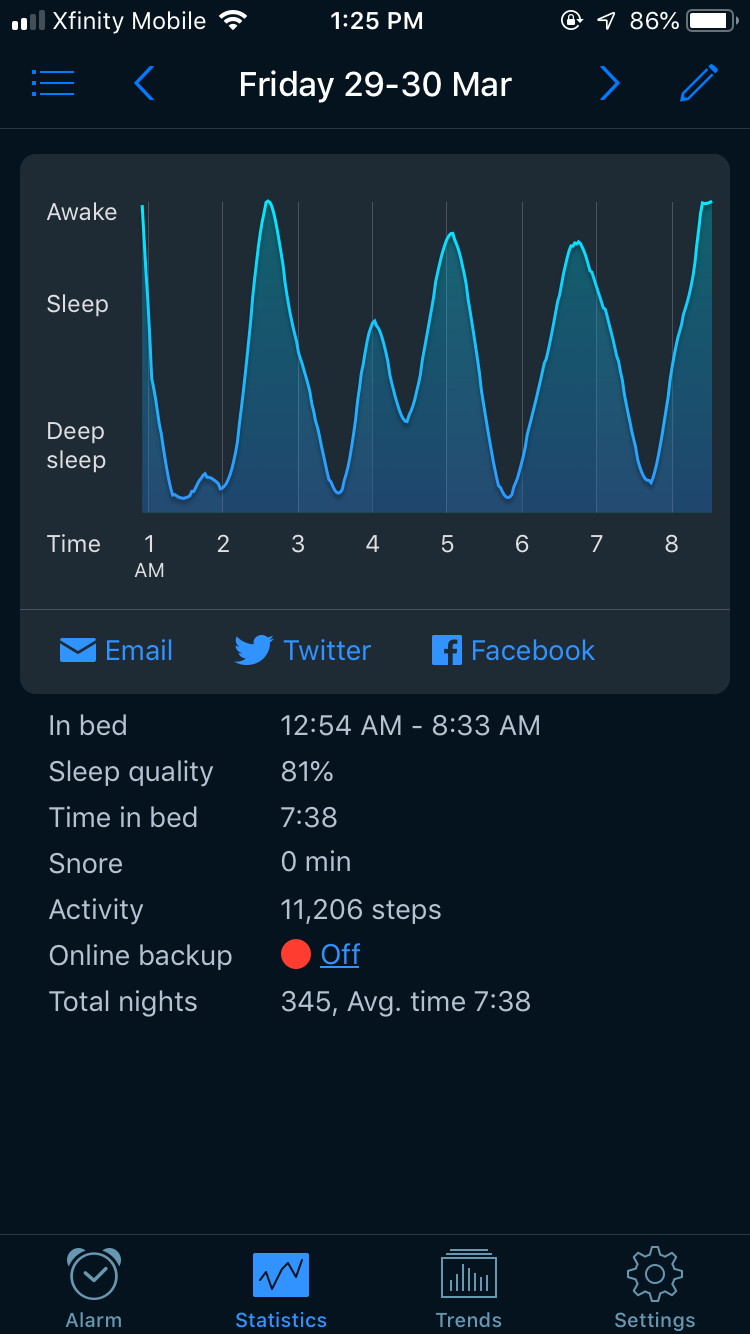
\includegraphics[width=0.25\linewidth]{img/example_night} 

}

\caption{Example night}\label{fig:example_night}
\end{figure}

One of these statistics is a ``Sleep Quality'' number, which is the
principle outcome variable in this experiment. According to the
\emph{Sleep Cycle} website, these four factors go into calculating Sleep
Quality:

\begin{enumerate}
\def\labelenumi{\arabic{enumi}.}
\tightlist
\item
  Amount of time spent in bed.
\item
  Amount of time spent in deep sleep.
\item
  Consistency of the sleep.
\item
  Amount of times where the app registered you as fully awake.
\end{enumerate}

Of the four factors, users generally only have direct control over the
first one. In order to be less intrusive, we did not control the amount
of time that users spend in bed, but we did instruct subjects to try to
sleep at regular hours every night. The other three factors are
hopefully affected by screen-time, allowing us to measure a treatment
effect. The app also records a ``snore'' and ``steps walked'' value, but
we have doubts about the accuracy of these measures and will not use
them in our analysis.

The experiment took place over two weeks, from March 23 to April 5 of
2019. Saturday was chosen as the start day of the week because it was
feared that instructions to change sleep habits in the middle of the
week might be ignored. We recruited 35 people for the study using a
Google survey, consisting of classmates, friends, and family. In
addition to asking for contact and demographic information, the survey
also inquired about general sleep habits such as bedtime and pre-sleep
activities. While the survey did ask about electronic usage, the
questions were mixed in among other questions such as workout habits and
alcohol consumption. Prior to commencement of the experiment, subjects
were not made aware of the fact that screen-time was the critical
variable of interest.

All communications to subjects occurred over email. Every person in the
same experimental group received identical emails (see Appendix). When
instructing subjects to use electronics prior to bed, we did not mandate
any specific activity, as we felt it would increase non-compliance on an
already-intrusive study. We only specified that users should use some
sort of electronic device with a backlit screen for 30 minutes
immediately before bedtime. Similarly, we did not ask subjects in the
other group to perform anything in lieu of electronic usage. These
subjects were simply asked to refrain from using electronics with
backlit screens 30 minutes before bedtime.

Subjects were assigned randomly to two groups, with group 1 receiving
treatment (screen-time before bed) during the first week and group 2
receiving control (no screen-time before bed). After the first week,
subjects were instructed to swap to the opposite activity of what they
were assigned to initially. The swapping design allows us to perform
within-subject comparisons while also leaving time for treatment effects
to manifest themselves. With the group that received treatment first, we
are also able to perform some analysis on persistence effects. Note that
subjects were not informed of the instruction swap ahead of time, so we
do not expect any anticipation effects.

The nature of experiment requires effort from subjects in both treatment
and control. That is, for people who normally use electronic devices
before bed, the request to refrain from usage constitutes a significant
change in pre-sleep ritual; for people who normally avoid electronics
before bed, the opposite is true. Therefore, we are concerned with
two-sided non-compliance, which is especially difficult to measure in
this experiment because people are unlikely to honestly report when they
have deviated from our instructions. To help combat this somewhat, we
offered subjects some small monetary compensation and emphasized
prioritization of honesty of compliance in reporting data. Even so, we
can never be sure of whether subjects followed instructions.

\subsection{Experiment Deviations}\label{experiment-deviations}

Between the closing the sign-up survey, we asked all respondents to
begin using the app in order to establish baseline data and help the app
calibrate (the website claims that the app becomes more accurate over
time). Sleep habits during this baseline usage were not closely
controlled or monitored, as each subject signed up for the experiment at
different dates. However, we did ask for an export of this baseline data
prior to starting the experiment, so that subjects had some awareness of
the steps it takes to perform the export. At this time, we learned that
Android users could not perform the export due to missing functionality
in the app. As such, we asked Android users (4 out of the 38) to
manually record the sleep times and quality from the app each day.

After closing the sign-up survey, we decided to also included ourselves
as subjects in the experiment. This was to slightly raise the number of
subjects and out of curiosity for the effects on ourselves. Though we
were not aware of our own randomization a priori, we obviously had more
knowledge of the experiment than other subjects, so we will analyze our
own data with special care.

\section{Results}\label{results}

\subsection{Data Cleaning}\label{data-cleaning}

We made as little modification to the raw data as possible, but a few
exceptions exist. We decided to omit entries for which the subject slept
for a duration shorter than one hour. On case by case basis, we
determined that these entries were caused by improper usage of the app.
There were several entries where the user had two entries in one night,
separated by some period of awakeness. In these cases, one or both of
the periods of sleep were also very short. However, none of them fell
under the one hour threshold for omission.

Of the 38 people who originally signed up for the study, only 29 people
actually submitted final data by the time of writing this report. As
such, we excluded their results. Note that these subjects are not
necessarily attriters, as we could not collect data from treatment or
control.

\subsection{Analysis}\label{analysis}

Before presenting the analysis, it should be noted that this experiment
is very underpowered. It was difficult to recruit a significant number
of people who would agree to have their sleep monitored and controlled
over several weeks. For our \texttt{n} size of 29, to see a small effect
size (Cohen's \texttt{d\ =\ 0.2}) at the 0.05 significance level, we
only have a power of about 0.12.

\begin{figure}
\centering
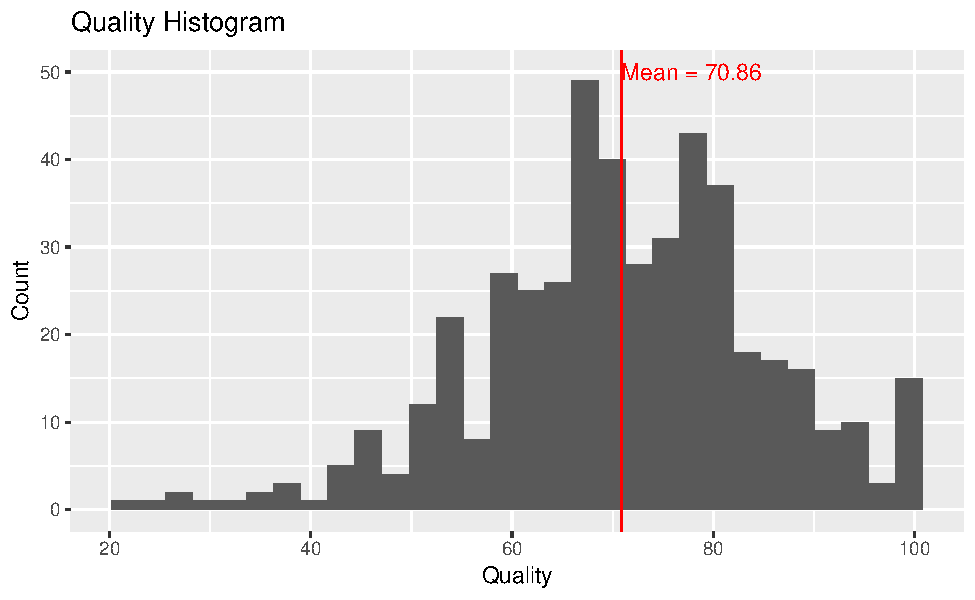
\includegraphics{report_files/figure-latex/quality_histogram-1.pdf}
\caption{\label{fig:quality_histogram} Quality histogram}
\end{figure}

Figure \ref{fig:quality_histogram} shows the distribution of the sleep
quality over the entire experiment. This includes data from the baseline
and actual experiment. We see a slight left skew, even after removing
the entries with fewer than one hour of sleep. There is also a slight
build up at 100 due to that being the maximum number that the app
reports. We do not believe that the peaks around 70 and 80 are special.

\begin{figure}
\centering
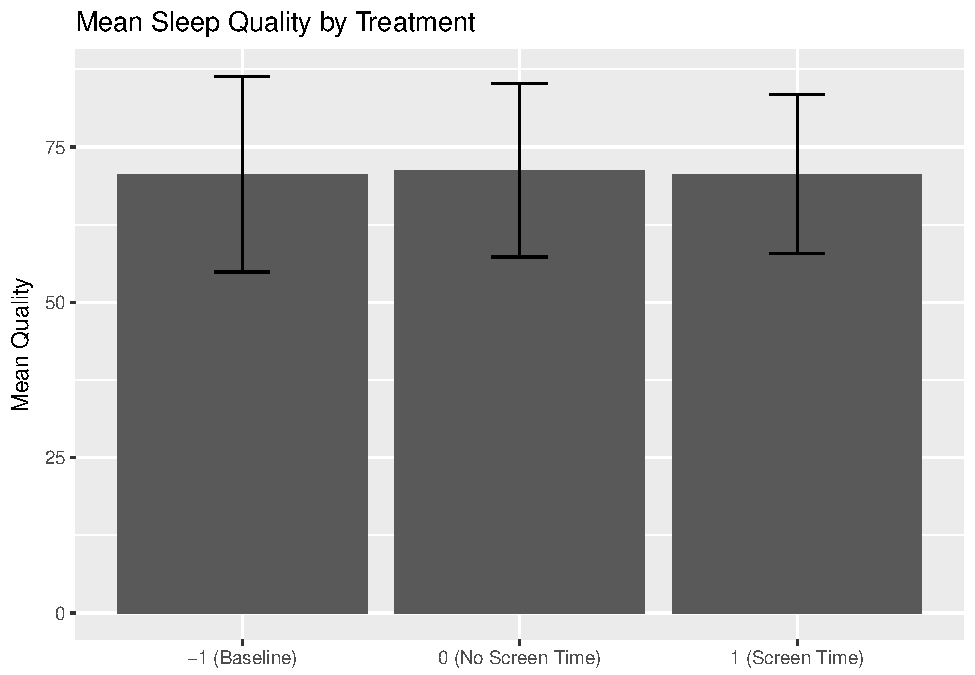
\includegraphics{report_files/figure-latex/quality_by_treatment_fig-1.pdf}
\caption{\label{fig:quality_by_treatment_fig} Mean sleep quality by
treatment}
\end{figure}

\begin{table}[!htbp] \centering 
  \caption{\label{tab:quality_by_treatment_tab} Mean sleep quality by treatment} 
  \label{} 
\begin{tabular}{@{\extracolsep{5pt}} ccc} 
\\[-1.8ex]\hline 
\hline \\[-1.8ex] 
Label & Mean & St. Err. \\ 
\hline \\[-1.8ex] 
Baseline & $70.608$ & $1.378$ \\ 
No Screen Time & $70.618$ & $1.022$ \\ 
Screen Time & $71.246$ & $1.042$ \\ 
\hline \\[-1.8ex] 
\end{tabular} 
\end{table}

Figure \ref{fig:quality_by_treatment_fig} shows the sleep quality,
averaged over the respective time periods, for each treatment
assignment. The reported error bars are standard error for each time
period. As mentioned above, the baseline data was collected in the time
between subjects signing up and the experiment officially starting. We
did not tightly control baseline data and not every subject provided it.

It is already clear that our experiment will not show the hypothesized
effect, as the point estimate for screen time is actually slightly
higher than that with no screen time. More importantly, the standard
errors completely dominate any difference between the treatments. Table
\ref{tab:quality_by_treatment_tab} shows the tabular results for Figure
\ref{fig:quality_by_treatment_fig}.

\begin{figure}
\centering
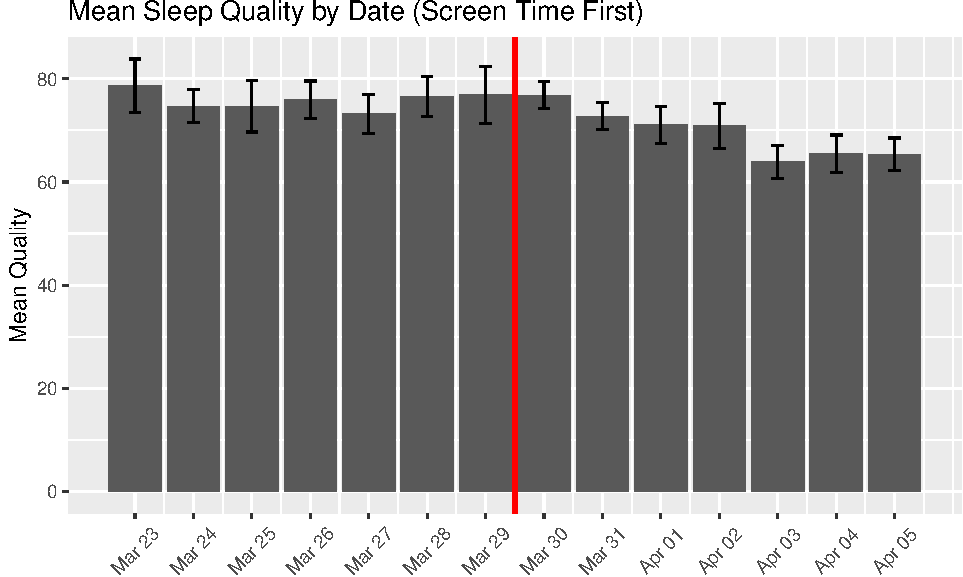
\includegraphics{report_files/figure-latex/quality_by_date_group1_fig-1.pdf}
\caption{\label{fig:quality_by_date_group1_fig} Mean sleep quality by
date in group which received screen time first}
\end{figure}

\begin{figure}
\centering
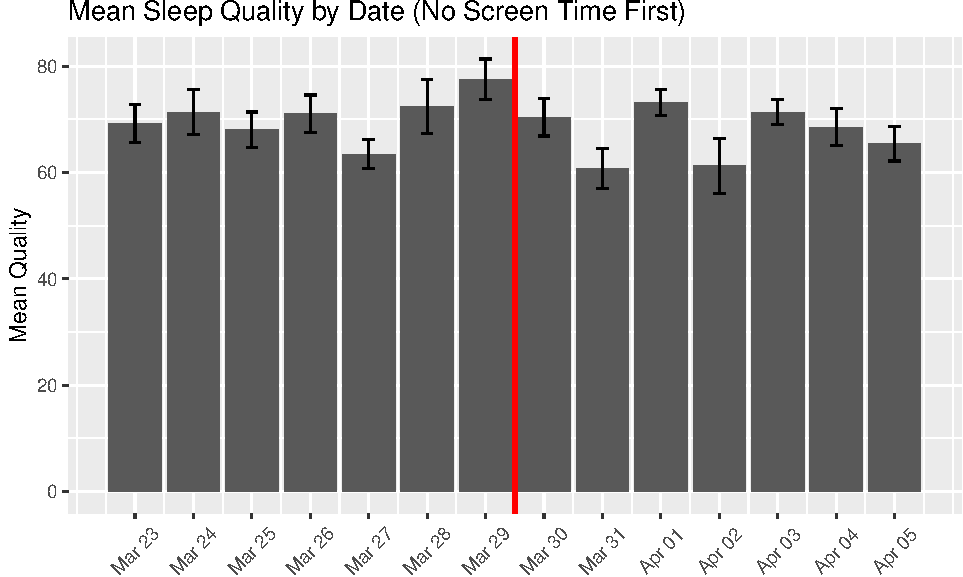
\includegraphics{report_files/figure-latex/quality_by_date_group2_fig-1.pdf}
\caption{\label{fig:quality_by_date_group2_fig} Mean sleep quality by
date in group that received no screen time first}
\end{figure}

Figure \ref{fig:quality_by_date_group1_fig} and Figure
\ref{fig:quality_by_date_group2_fig} show the mean sleep quality by
dates for the two groups. Recall that group 1 received treatment (screen
time) in week 1 of the experiment and switched to control (no screen
time) in week 2. Group 2 had the opposite schedule. Again, the large
error bars make it hard to draw any sort of conclusion for whether the
switch in treatment has any effect, but it could be argued that there is
a slight drop in quality in group 1, after they switch from screen time
to no screen time. Although still likely due to random noise, this drop
is probably what primarily drives the treatment point estimate being in
the opposite direction of the expected effect.

Table \ref{tab:quality_regressions} shows the results of three
regressions models:

\begin{enumerate}
\def\labelenumi{\arabic{enumi}.}
\tightlist
\item
  \(quality = \beta_0 + \beta_1 treat\)
\item
  \(quality = \beta_0 + \beta_1 treat + \sum_i \gamma_i id_i\)
\item
  \(quality = \beta_0 + \beta_1 treat + \sum_j \delta_j x_j\)
\end{enumerate}

In model 1, we naively regress on just the treatment variable. This
yields the 0.628 point effect that was already shown in Table
\ref{tab:quality_by_treatment_tab}. However, we are not taking into the
account that multiple entries in the dataset came from the same person.

We assigned a numerical ID to each participant in the study. This
provides a unique indicator variable for each person and the standard
errors reported in Table \ref{tab:quality_regressions} are actually
clustered standard errors based on those IDs. In model 2, we control for
the fixed effects to each person. This brings down the treatment effect
(which was already statistically insignificant) even closer to zero.

Recall that the sign-up form for the experiment also contained several
questions regarding sleep habits. In model 3, we regress on these in
lieu of the subject IDs. See the pre-experiment survey in the appendix
for the list of covariates. The self-reported bedtime stands out as a
variable that is highly statistically significant. We will not draw any
causal inference from this fact, as we did not randomize subjects'
bedtimes. It is also important to reiterate that these are not the
actual observed bed times in the experiment, but the estimated bed time
that subjects reported in the pre-experiment survey. However, it does
seem that for this group of people, self-reported late sleepers also
have higher sleep quality. In addition, we are surprised that whether or
not a subject shared a bed with a partner did not have even higher
statistical significance. Unless both people are simultaneously using
the app, \emph{Sleep Cycle} cannot distinguish movement from one person
or another. It should be the case that multiple people should make much
more noise and trick the app into thinking that its user is awake for
longer than actuality.

\begin{table}[!htbp] \centering 
  \caption{\label{tab:quality_regressions} Regressions, outcome is sleep quality} 
  \label{} 
\begin{tabular}{@{\extracolsep{5pt}}lccc} 
\\[-1.8ex]\hline 
\hline \\[-1.8ex] 
 & \multicolumn{3}{c}{\textit{Dependent variable:}} \\ 
\cline{2-4} 
\\[-1.8ex] & \multicolumn{3}{c}{Sleep Quality} \\ 
\\[-1.8ex] & (1) & (2) & (3)\\ 
\hline \\[-1.8ex] 
 Treatment (Screen-time) & 0.628 & 0.120 & $-$0.394 \\ 
  & (1.581) & (1.639) & (1.637) \\ 
  & & & \\ 
 Age &  &  & 0.276 \\ 
  &  &  & (0.206) \\ 
  & & & \\ 
 Male &  &  & 1.376 \\ 
  &  &  & (3.175) \\ 
  & & & \\ 
 Bed time &  &  & 0.402$^{***}$ \\ 
  &  &  & (0.140) \\ 
  & & & \\ 
 Rise time &  &  & 0.587 \\ 
  &  &  & (1.637) \\ 
  & & & \\ 
 Daily caffeine &  &  & $-$1.507$^{*}$ \\ 
  &  &  & (0.915) \\ 
  & & & \\ 
 Workout close to bedtime &  &  & $-$0.641 \\ 
  &  &  & (2.558) \\ 
  & & & \\ 
 Daily electronics use &  &  & $-$0.036 \\ 
  &  &  & (0.313) \\ 
  & & & \\ 
 Electronics stop before bed &  &  & 0.027 \\ 
  &  &  & (0.107) \\ 
  & & & \\ 
 King Size Bed &  &  & 4.117 \\ 
  &  &  & (3.729) \\ 
  & & & \\ 
 Queen Size Bed &  &  & $-$4.652$^{*}$ \\ 
  &  &  & (2.790) \\ 
  & & & \\ 
 Twin Size Bed &  &  & 4.276 \\ 
  &  &  & (3.541) \\ 
  & & & \\ 
 Shares bed &  &  & $-$8.919$^{*}$ \\ 
  &  &  & (4.757) \\ 
  & & & \\ 
 Constant & 70.618$^{***}$ & 71.940$^{***}$ & 58.968$^{***}$ \\ 
  & (1.564) & (0.819) & (19.061) \\ 
  & & & \\ 
\hline \\[-1.8ex] 
Control for user ID & No & Yes & No \\ 
Observations & 336 & 336 & 326 \\ 
R$^{2}$ & 0.001 & 0.297 & 0.146 \\ 
Adjusted R$^{2}$ & $-$0.002 & 0.231 & 0.110 \\ 
Residual Std. Error & 13.424 (df = 334) & 11.761 (df = 306) & 12.571 (df = 312) \\ 
F Statistic & 0.183 (df = 1; 334) & 4.460$^{***}$ (df = 29; 306) & 4.087$^{***}$ (df = 13; 312) \\ 
\hline 
\hline \\[-1.8ex] 
\textit{Note:}  & \multicolumn{3}{r}{$^{*}$p$<$0.1; $^{**}$p$<$0.05; $^{***}$p$<$0.01} \\ 
\end{tabular} 
\end{table}

\begin{figure}
\centering
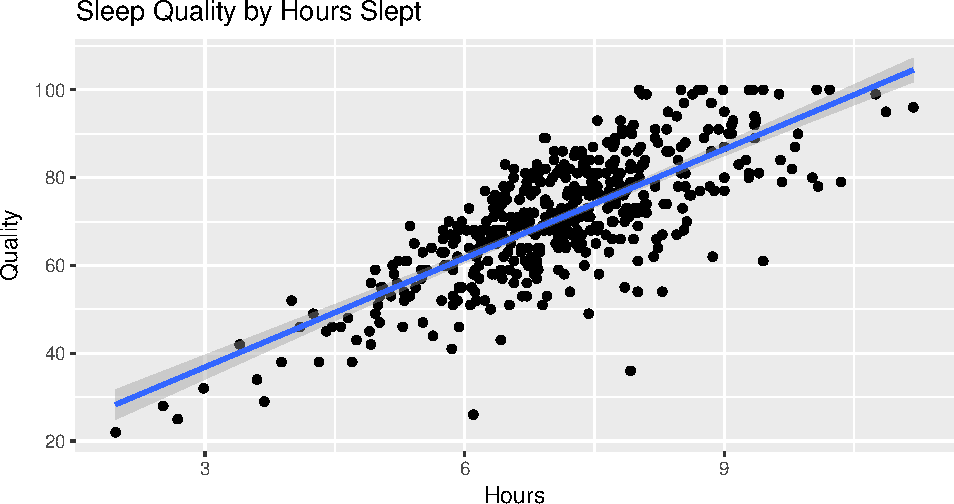
\includegraphics{report_files/figure-latex/quality_by_hours_fig-1.pdf}
\caption{\label{fig:quality_by_hours_fig} Mean sleep quality by hours
slept}
\end{figure}

Figure \ref{fig:quality_by_hours_fig} shows that sleep quality is highly
correlated hours slept. Table \ref{tab:quality_hours_regression} shows
the strength of this relationship. Since these two variables are so
predictive of one-another, it may be interesting to also use hours slept
as an outcome variable.

\begin{table}[!htbp] \centering 
  \caption{\label{tab:quality_hours_regression} Regression, quality on hours} 
  \label{} 
\begin{tabular}{@{\extracolsep{5pt}}lc} 
\\[-1.8ex]\hline 
\hline \\[-1.8ex] 
 & \multicolumn{1}{c}{\textit{Dependent variable:}} \\ 
\cline{2-2} 
\\[-1.8ex] & quality \\ 
\hline \\[-1.8ex] 
 Hours & 8.268$^{***}$ \\ 
  & (0.396) \\ 
  & \\ 
 Constant & 12.060$^{***}$ \\ 
  & (2.853) \\ 
  & \\ 
\hline \\[-1.8ex] 
Observations & 466 \\ 
R$^{2}$ & 0.584 \\ 
Adjusted R$^{2}$ & 0.583 \\ 
Residual Std. Error & 9.088 (df = 464) \\ 
F Statistic & 650.944$^{***}$ (df = 1; 464) \\ 
\hline 
\hline \\[-1.8ex] 
\textit{Note:}  & \multicolumn{1}{r}{$^{*}$p$<$0.1; $^{**}$p$<$0.05; $^{***}$p$<$0.01} \\ 
\end{tabular} 
\end{table}

Thus, we run the analogous three regression to Table
\ref{tab:quality_regressions}. Table \ref{tab:hours_regressions} shows
the results. Again, we see no statistically significant treatment
effects. However, the bed time coefficient is still significant. It is
worth investigating this further.

\begin{table}[!htbp] \centering 
  \caption{\label{tab:hours_regressions} Regressions, outcome is hours slept} 
  \label{} 
\begin{tabular}{@{\extracolsep{5pt}}lccc} 
\\[-1.8ex]\hline 
\hline \\[-1.8ex] 
 & \multicolumn{3}{c}{\textit{Dependent variable:}} \\ 
\cline{2-4} 
\\[-1.8ex] & \multicolumn{3}{c}{Hours Slept} \\ 
\\[-1.8ex] & (1) & (2) & (3)\\ 
\hline \\[-1.8ex] 
 Treatment (Screen-time) & 0.123 & 0.088 & 0.036 \\ 
  & (0.126) & (0.138) & (0.143) \\ 
  & & & \\ 
 Age &  &  & 0.045$^{**}$ \\ 
  &  &  & (0.023) \\ 
  & & & \\ 
 Male &  &  & 0.245 \\ 
  &  &  & (0.313) \\ 
  & & & \\ 
 Bed time &  &  & 0.042$^{**}$ \\ 
  &  &  & (0.018) \\ 
  & & & \\ 
 Rise time &  &  & 0.198 \\ 
  &  &  & (0.197) \\ 
  & & & \\ 
 Daily caffeine &  &  & $-$0.074 \\ 
  &  &  & (0.118) \\ 
  & & & \\ 
 Workout close to bedtime &  &  & $-$0.318 \\ 
  &  &  & (0.233) \\ 
  & & & \\ 
 Daily electronics use &  &  & $-$0.0001 \\ 
  &  &  & (0.033) \\ 
  & & & \\ 
 Electronics stop before bed &  &  & 0.005 \\ 
  &  &  & (0.012) \\ 
  & & & \\ 
 King Size Bed &  &  & 0.299 \\ 
  &  &  & (0.467) \\ 
  & & & \\ 
 Queen Size Bed &  &  & $-$0.544 \\ 
  &  &  & (0.361) \\ 
  & & & \\ 
 Twin Size Bed &  &  & 0.984$^{**}$ \\ 
  &  &  & (0.428) \\ 
  & & & \\ 
 Shares bed &  &  & $-$0.900$^{*}$ \\ 
  &  &  & (0.534) \\ 
  & & & \\ 
 Constant & 7.054$^{***}$ & 7.272$^{***}$ & 4.149$^{*}$ \\ 
  & (0.157) & (0.069) & (2.166) \\ 
  & & & \\ 
\hline \\[-1.8ex] 
Control for user ID & No & Yes & No \\ 
Observations & 336 & 336 & 326 \\ 
R$^{2}$ & 0.002 & 0.398 & 0.177 \\ 
Adjusted R$^{2}$ & $-$0.001 & 0.341 & 0.143 \\ 
Residual Std. Error & 1.243 (df = 334) & 1.009 (df = 306) & 1.149 (df = 312) \\ 
F Statistic & 0.819 (df = 1; 334) & 6.988$^{***}$ (df = 29; 306) & 5.169$^{***}$ (df = 13; 312) \\ 
\hline 
\hline \\[-1.8ex] 
\textit{Note:}  & \multicolumn{3}{r}{$^{*}$p$<$0.1; $^{**}$p$<$0.05; $^{***}$p$<$0.01} \\ 
\end{tabular} 
\end{table}

\subsection{Non-compliance}\label{non-compliance}

\begin{figure}
\centering
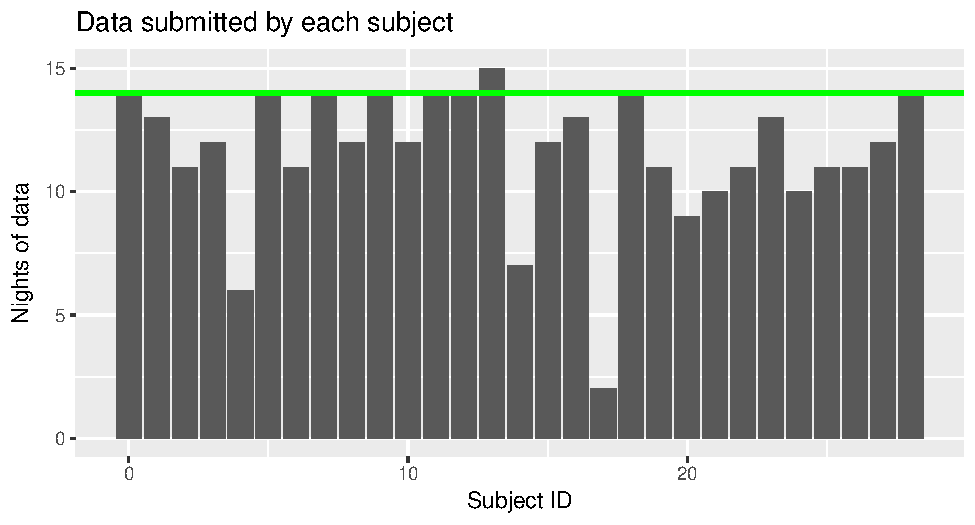
\includegraphics{report_files/figure-latex/days_used-1.pdf}
\caption{\label{fig:days_used} Number of nights of data submitted by
each participant}
\end{figure}

Non-compliance was major issue in this experiment. Beyond not following
our instructions on electronics usage, many subjects simply did not use
the app. Figure \ref{fig:days_used} shows the number of nights of data
that each subject actually submitted. The experiment took place over two
weeks and ideally we would have received 14 nights of data from each
person. Clearly this was not the case. The mean number of nights
submitted was just 11.6 days, with one participant only using the app
for 2 out of the 14 nights. As an aside, the one subject with 15 nights
of data used the app twice in one night. The subject went to sleep, woke
up, and then went to sleep again.

\section{Conclusion}\label{conclusion}

Through our findings and analysis of the data we reject our hypothesis
that there is statistical significance between thirty minutes of screen
time before going to bed and sleep quality. Additionally we fail to
reject the null hypothesis which suggests that there is no statistical
significance between screen time thirty minutes before going to bed and
dleep quality.

This experiment was too small to demonstrate any statistically
significant treatment effect. It would be interesting to repeat this
test with a much larger population.


\end{document}
